\subsection*{Adding perturbations}

We are now going to introduce some noise on the measured data. So our vector $f$ is redefined for $i=1,...,36$ by :
\begin{align*}
f_i&=f(y_i)+g_i 
\end{align*}

Where $g_i$'s come from a normal distribution with standard deviation 0.01. 

The Matlab code $svdPert.m$ (available at the end of the report) contains the code used to obtain the plots presented here.

\begin{figure}
\begin{center}
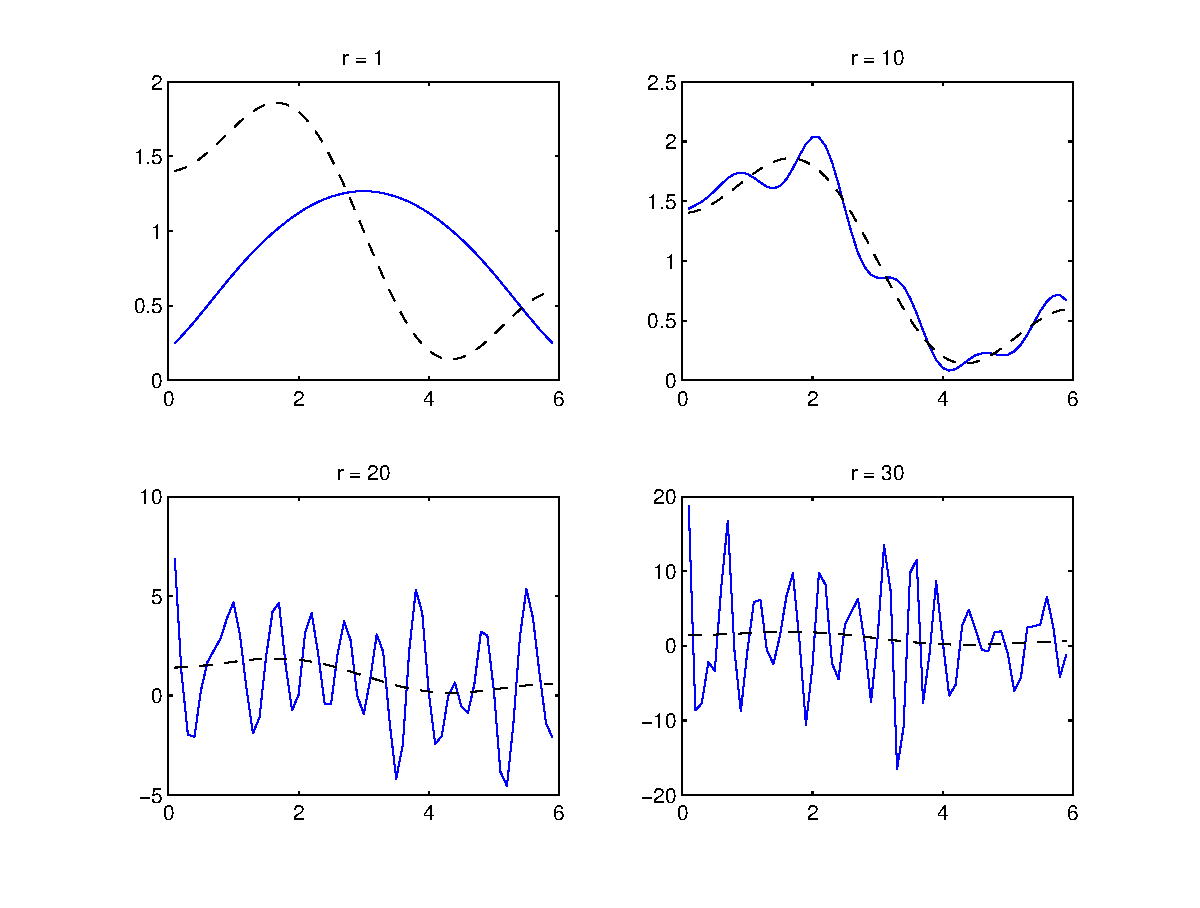
\includegraphics[scale=0.6]{perturb.eps}
\caption{Results for some values of $r$ with perturbations}
\label{perturb}
\end{center}
\end{figure}

Figure \ref{perturb} shows the solution computed with the same values of $r$ as for the problem without any perturbation. Comparing to figure \ref{fig:nn1}, we can see that for the lower values of $r$ ($r=1$ or $r=10$), the approximation is quite similar. 

On the other hand, for $r=20$ and $r=30$, adding perturbations greatly affect the quality of the solution. This is because the problem is ill-posed and thus small variations on the vector $f$ will greatly influence the solution.

Because of the perturbations, we feel, after looking at graphs for different ranks $r$, that the "best" approximation is when $r=7$. Figure \ref{rank7} shows the plot.

\begin{figure}
\begin{center}
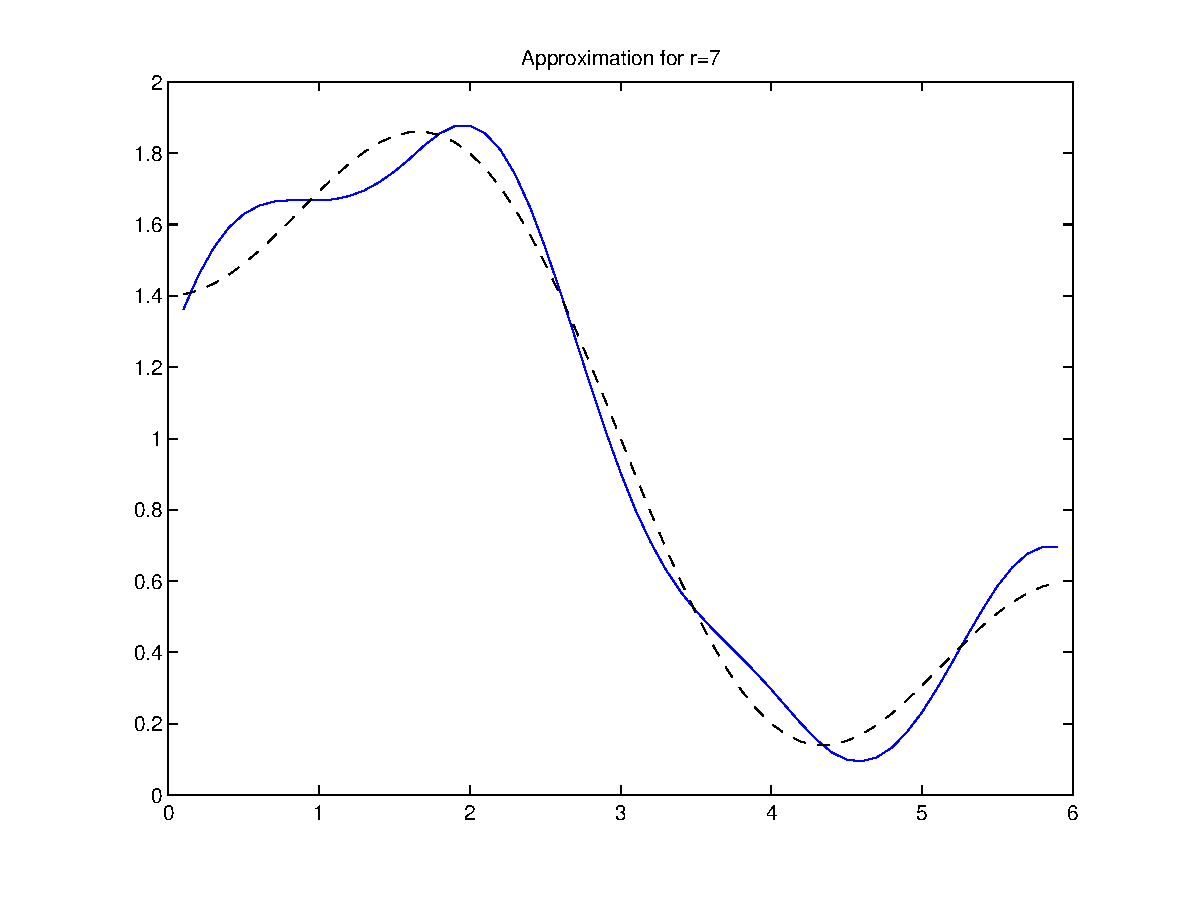
\includegraphics[scale=0.7]{rank7.eps}
\caption{Approximation for $r=7$}
\label{rank7}
\end{center}
\end{figure} 

We can note here that, because $r=7$, we are only using 7 singular values (out of the 36 possible!). Although this might seem low, we can see that the approximation is quite good.